\chapter{Конструкторская часть}

В данном разделе будут рассмотрены схемы вышеизложенных алгоритмов, а также вычислена их трудоемкость.

\section{Разработка алгоритмов}

На рисунке \ref{img:classic} представлен классический алгоритм умножения матриц.

\begin{figure}[H]
	\begin{center}
		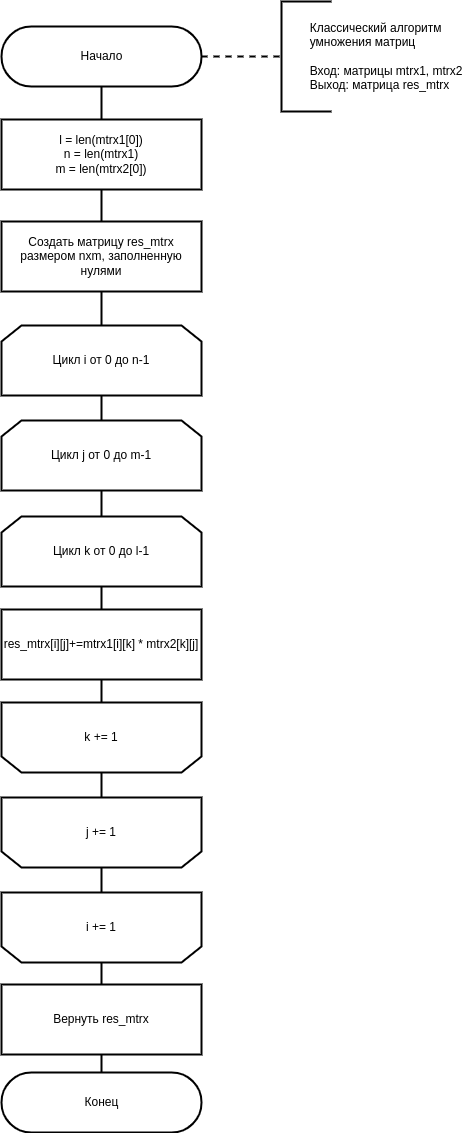
\includegraphics[scale=0.61]{img/classic.png}
	\end{center}
	\captionsetup{justification=centering}
	\caption{Схема классического алгоритма умножения матриц}
	\label{img:classic}
\end{figure}

На рисунке \ref{img:winograd} представлен алгоритм Винограда.

\begin{figure}[H]
	\begin{center}
		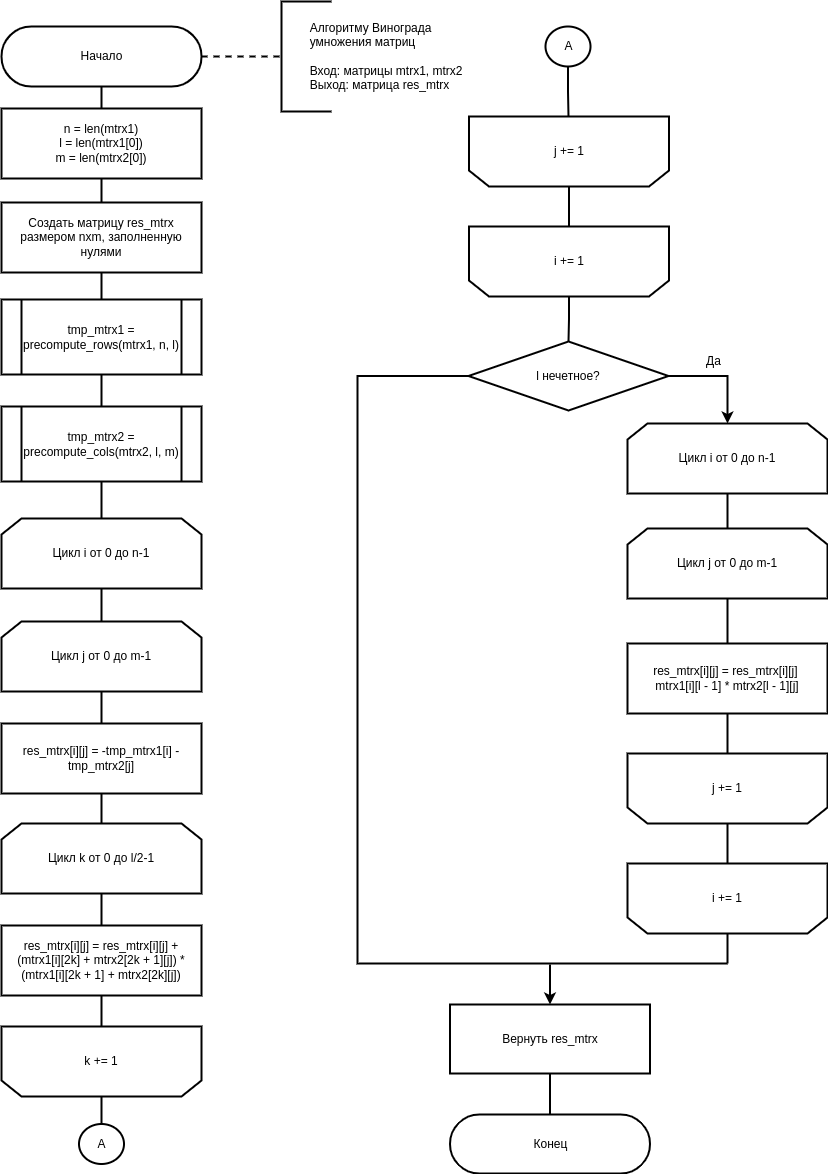
\includegraphics[scale=0.56]{img/winograd.png}
	\end{center}
	\captionsetup{justification=centering}
	\caption{Схема алгоритма Винограда}
	\label{img:winograd}
\end{figure}

На рисунке \ref{img:winograd_precompute} представлены алгоритмы предварительных вычислений слагаемых для алгоритма Винограда.

\begin{figure}[H]
	\begin{center}
		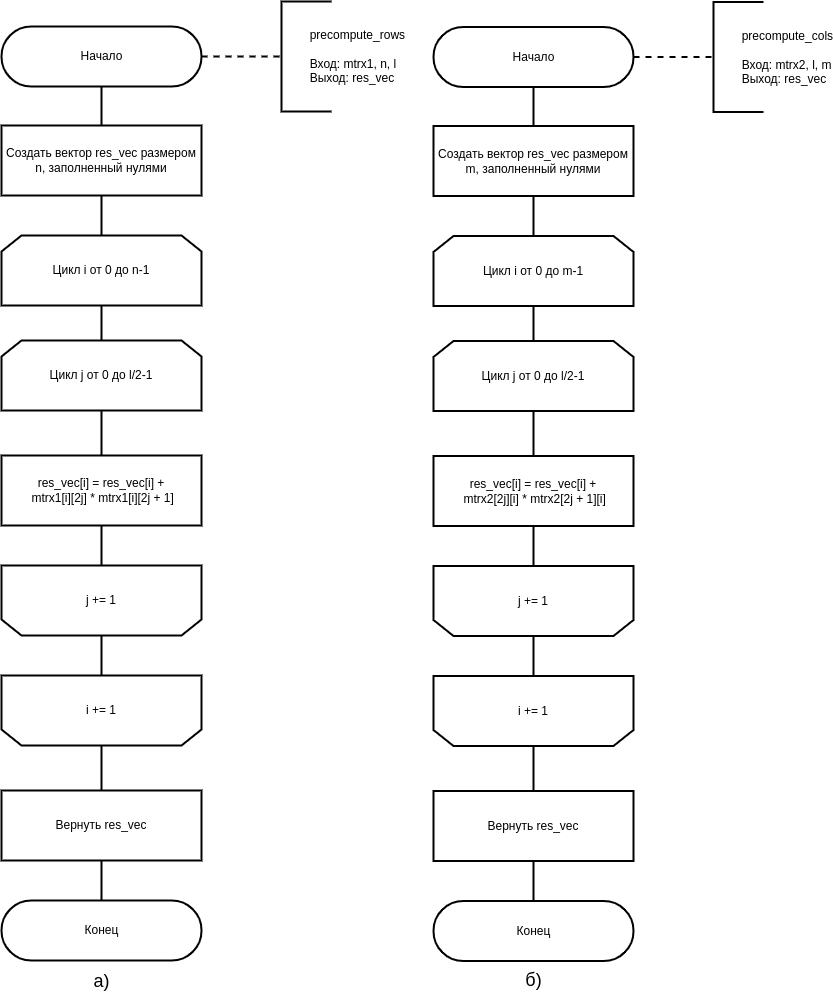
\includegraphics[scale=0.6]{img/winograd_precompute.png}
	\end{center}
	\captionsetup{justification=centering}
	\caption{Схемы алгоритмов предварительных вычислений слагаемых для алгоритма Винограда: а)для строк первой матрицы; б)для столбцов второй матрицы}
	\label{img:winograd_precompute}
\end{figure}

На рисунке \ref{img:optimized_winograd} представлен алгоритм Винограда с оптимизациями.

\begin{figure}[H]
	\begin{center}
		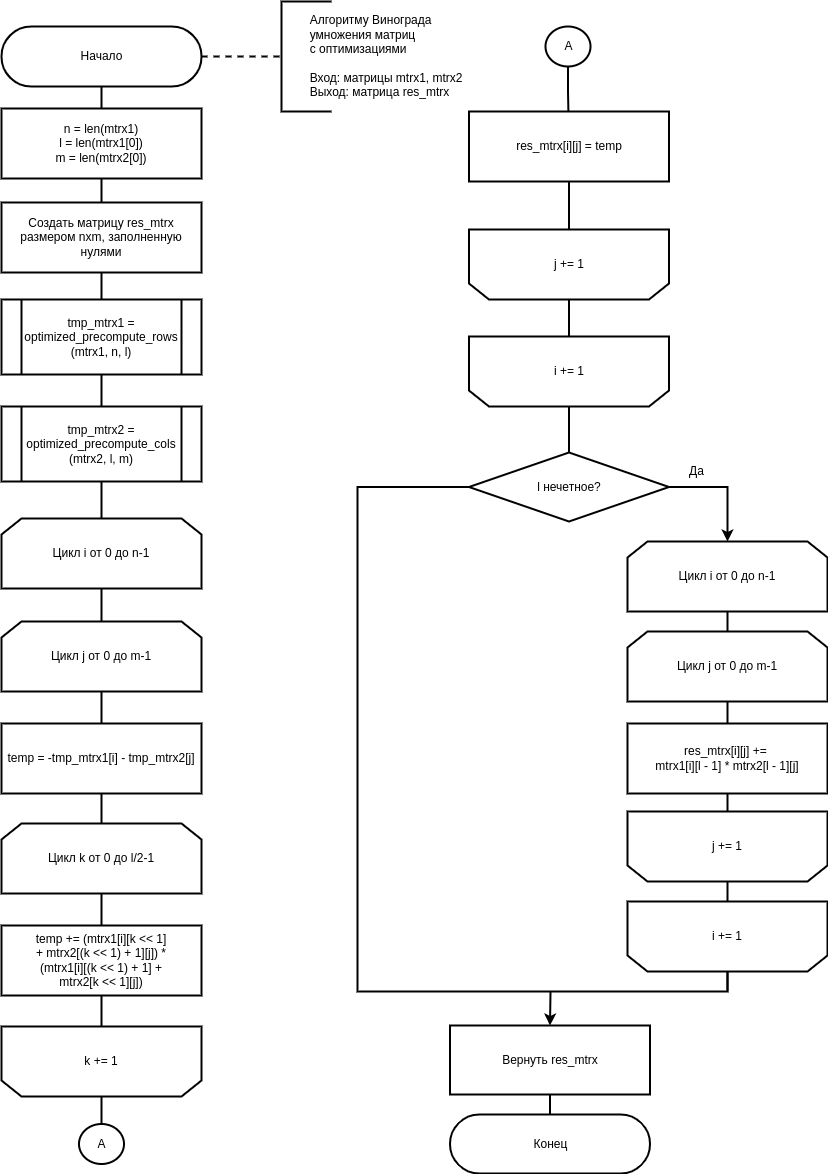
\includegraphics[scale=0.56]{img/optimized_winograd.png}
	\end{center}
	\captionsetup{justification=centering}
	\caption{Схема алгоритма Винограда с оптимизациями}
	\label{img:optimized_winograd}
\end{figure}

На рисунке \ref{img:optimized_winograd_precompute} представлены алгоритмы предварительных вычислений слагаемых для алгоритма Винограда с оптимизациями.

\begin{figure}[H]
	\begin{center}
		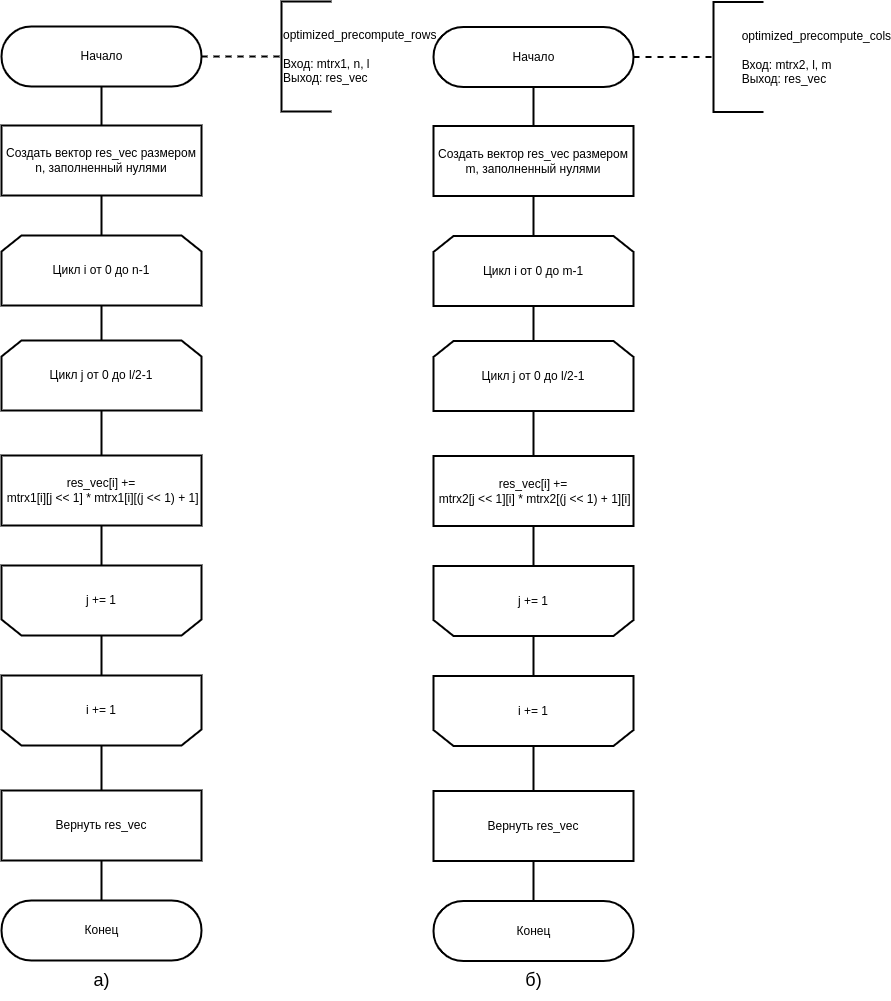
\includegraphics[scale=0.57]{img/optimized_winograd_precompute.png}
	\end{center}
	\captionsetup{justification=centering}
	\caption{Схемы алгоритмов предварительных вычислений слагаемых для алгоритма Винограда с оптимизациями:
		а)для строк первой матрицы; б)для столбцов второй матрицы}
	\label{img:optimized_winograd_precompute}
\end{figure}

\section{Вычисление трудоемкости алгоритмов}

\subsection{Классический алгоритм умножения матриц}

Трудоёмкость классического алгоритма равна (\ref{for:classic}):
\begin{equation}
	\label{for:classic}
	\begin{array}{c}
	f_{classic} = 2 + n \cdot (2 + 2 + m \cdot (2 + 2 + l \cdot 11)) = \\ 2 + 4 \cdot n + 4 \cdot mn + 11 \cdot lmn \approx 11 \cdot lmn
	\end{array}
\end{equation}

\subsection{Алгоритм Винограда}

Трудоёмкость алгоритма Винограда равна (\ref{for:winograd}):
\begin{equation}
	\label{for:winograd}
	\begin{array}{c}
	f_{winograd} = 2 + n \cdot (4 + 2 + l/2 \cdot 19) + 2 + l \cdot (4 + 2 + m/2 \cdot 19) +\\ 2 + n \cdot (2 + 2 + m \cdot (7 + 4 + 2 + l/2 \cdot 32)) + \\ 3 + \left[
	\begin{array}{c}
	0, \text{ лучший случай (размерность четная)}\\
	2 + n \cdot (2 + 2 + m \cdot 16), \text{ худший случай (нечетная)}\\
	\end{array}\right.\\
	= 9 + 10n + 6l + 19/2ln + 19/2lm + 13mn + 16lmn + \\ \left[
	\begin{array}{c}
		0, \text{ л. с.}\\
		2 + 4n + 16mn, \text{ х. с.}\\
	\end{array}\right.\\ \approx 16lmn
	\end{array}
\end{equation}

\subsection{Оптимизированный алгоритм Винограда}

Трудоёмкость оптимизированного алгоритма Винограда равна (\ref{for:optimized_winograd}):
\begin{equation}
	\label{for:optimized_winograd}
	\begin{array}{c}
		f_{optimized\_winograd} = 2 + n \cdot (4 + 2 + l/2 \cdot 15) + 2 + \\l \cdot (4 + 2 + m/2 \cdot 15) + 2 + \\n \cdot (2 + 2 + m \cdot (8 + 4 + 2 + l/2 \cdot 19)) + 3 + \\\left[
		\begin{array}{c}
			0, \text{ лучший случай (размерность четная)}\\
			2 + n \cdot (2 + 2 + m \cdot 13), \text{худший случай (нечетная)}\\
		\end{array}\right.\\
		= 9 + 10n + 6l + 15/2ln + 15/2lm + 14mn \\ 19/2lmn + \left[
		\begin{array}{c}
			0, \text{ л. с.}\\
			2 + 4n + 13mn, \text{ х. с.}\\
		\end{array}\right.\\ \approx 9,5lmn
	\end{array}
\end{equation}

\section*{Вывод}

На основе теоретических данных, полученных из аналитического раздела
были построены схемы требуемых алгоритмов. Кроме того, была произведена оценка трудоемкости алгоритмов. Наименее трудоемким алгоритмом оказался оптимизированный алгоритм Винограда.
